\documentclass[10pt, a4paper]{article}
\usepackage[T1]{fontenc}
\usepackage[utf8]{inputenc}
\usepackage{enumerate}
%\usepackage[swedish]{babel}
\usepackage{ifpdf}
\usepackage[parfill]{parskip}
\usepackage{graphicx}
\usepackage{fancyvrb}   % For source code listing.
\fvset{tabsize=4}       % Tabstop is 4 spaces.
\fvset{fontsize=\small} % Small fonts for source code.

\title{EDA031 Project - News System}
%\date{}
\author{
	\begin{tabular}{l l}
		Erik Westrup & \texttt{<ada09ewe@student.lu.se>}\\
		Joachim Nelson & \texttt{<ada08jne@student.lu.se>} \\ % TODO rätt mail?
		Oscar Olsson & \texttt{<ada09ool@student.lu.se>}
	\end{tabular}
}

\begin{document}

\begin{titlepage}
\maketitle
\thispagestyle{empty}	% No page number on title page.
\end{titlepage}
%\setcounter{page}{2}

\section{EDA031 Project - News System}
The purpose of the project was to develop a simple news system consisting of a client and server model. The objects of interest for the user is news articles. An article is have a title, is written by an author and contains text content. Articles are created by users using a client and are posted to different news groups. Each article belongs to one news group and are stored in a database at the server side. In total, the allowed operations from the users are listing news groups, listing articles in a specified news group, reading an article, creating articles, deleting articles and news groups.

The server was required to have a memory database and a persistent file database. The file database was implemented with one directory on disk for each news group and the articles as text files in these directories. The communication between the server and client uses a specified protocol in the application layer on top of TCP/IP. The server needed not be be multi-threaded but should sequentially be able to handle multiple clients.

\section{Detailed description of design and UML}
From the beginning we realized that the server and client will share much of the functionality related to network communication and data representation. We decided to make a net package containing classes dealing with communication. The package should of course be independent of client and server. Early on we also discussed if the information (result to queries)  at the server side could be reused at the client side. Later in the project this led to a database package DB containing both queries and the accompanying results that can be used on either side of the communication. However only one side needs to know how to send queries and the other how to receive and the reverse situation for the results. These parts was therefore split in and put at the server and client packages.

To meet the requirement of two databases we decided it would be best to make a database interface and to implemented that in a file and memory version. Our initial design is show in figure \ref{init+design}.

\begin{figure}[hbt]
\begin{center}
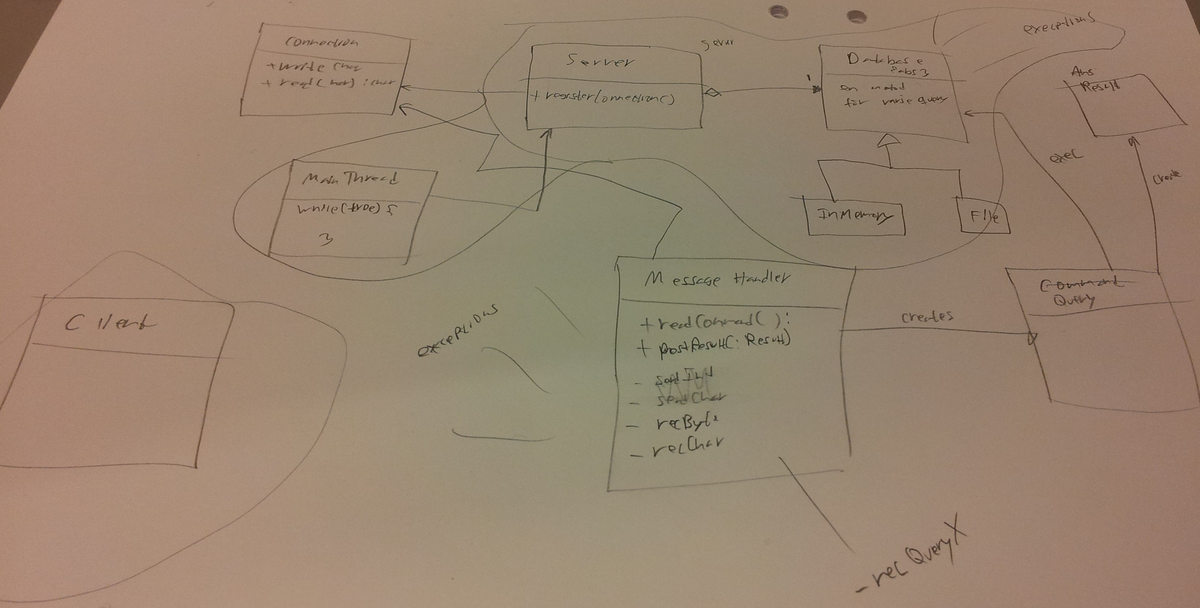
\includegraphics[scale=0.38]{img/uml_blueprint.png}
\end{center}
\label{init+design}
\caption{Initial design after our first project meeting.}
\end{figure}

In the final version of the system we had not deviated too much from the original design. The main difference is the previously mentioned separation of receiving and sending queries and results. A UML diagram of the final design can be seen in figure \ref{UML}.

\begin{figure}[hbt]
\begin{center}
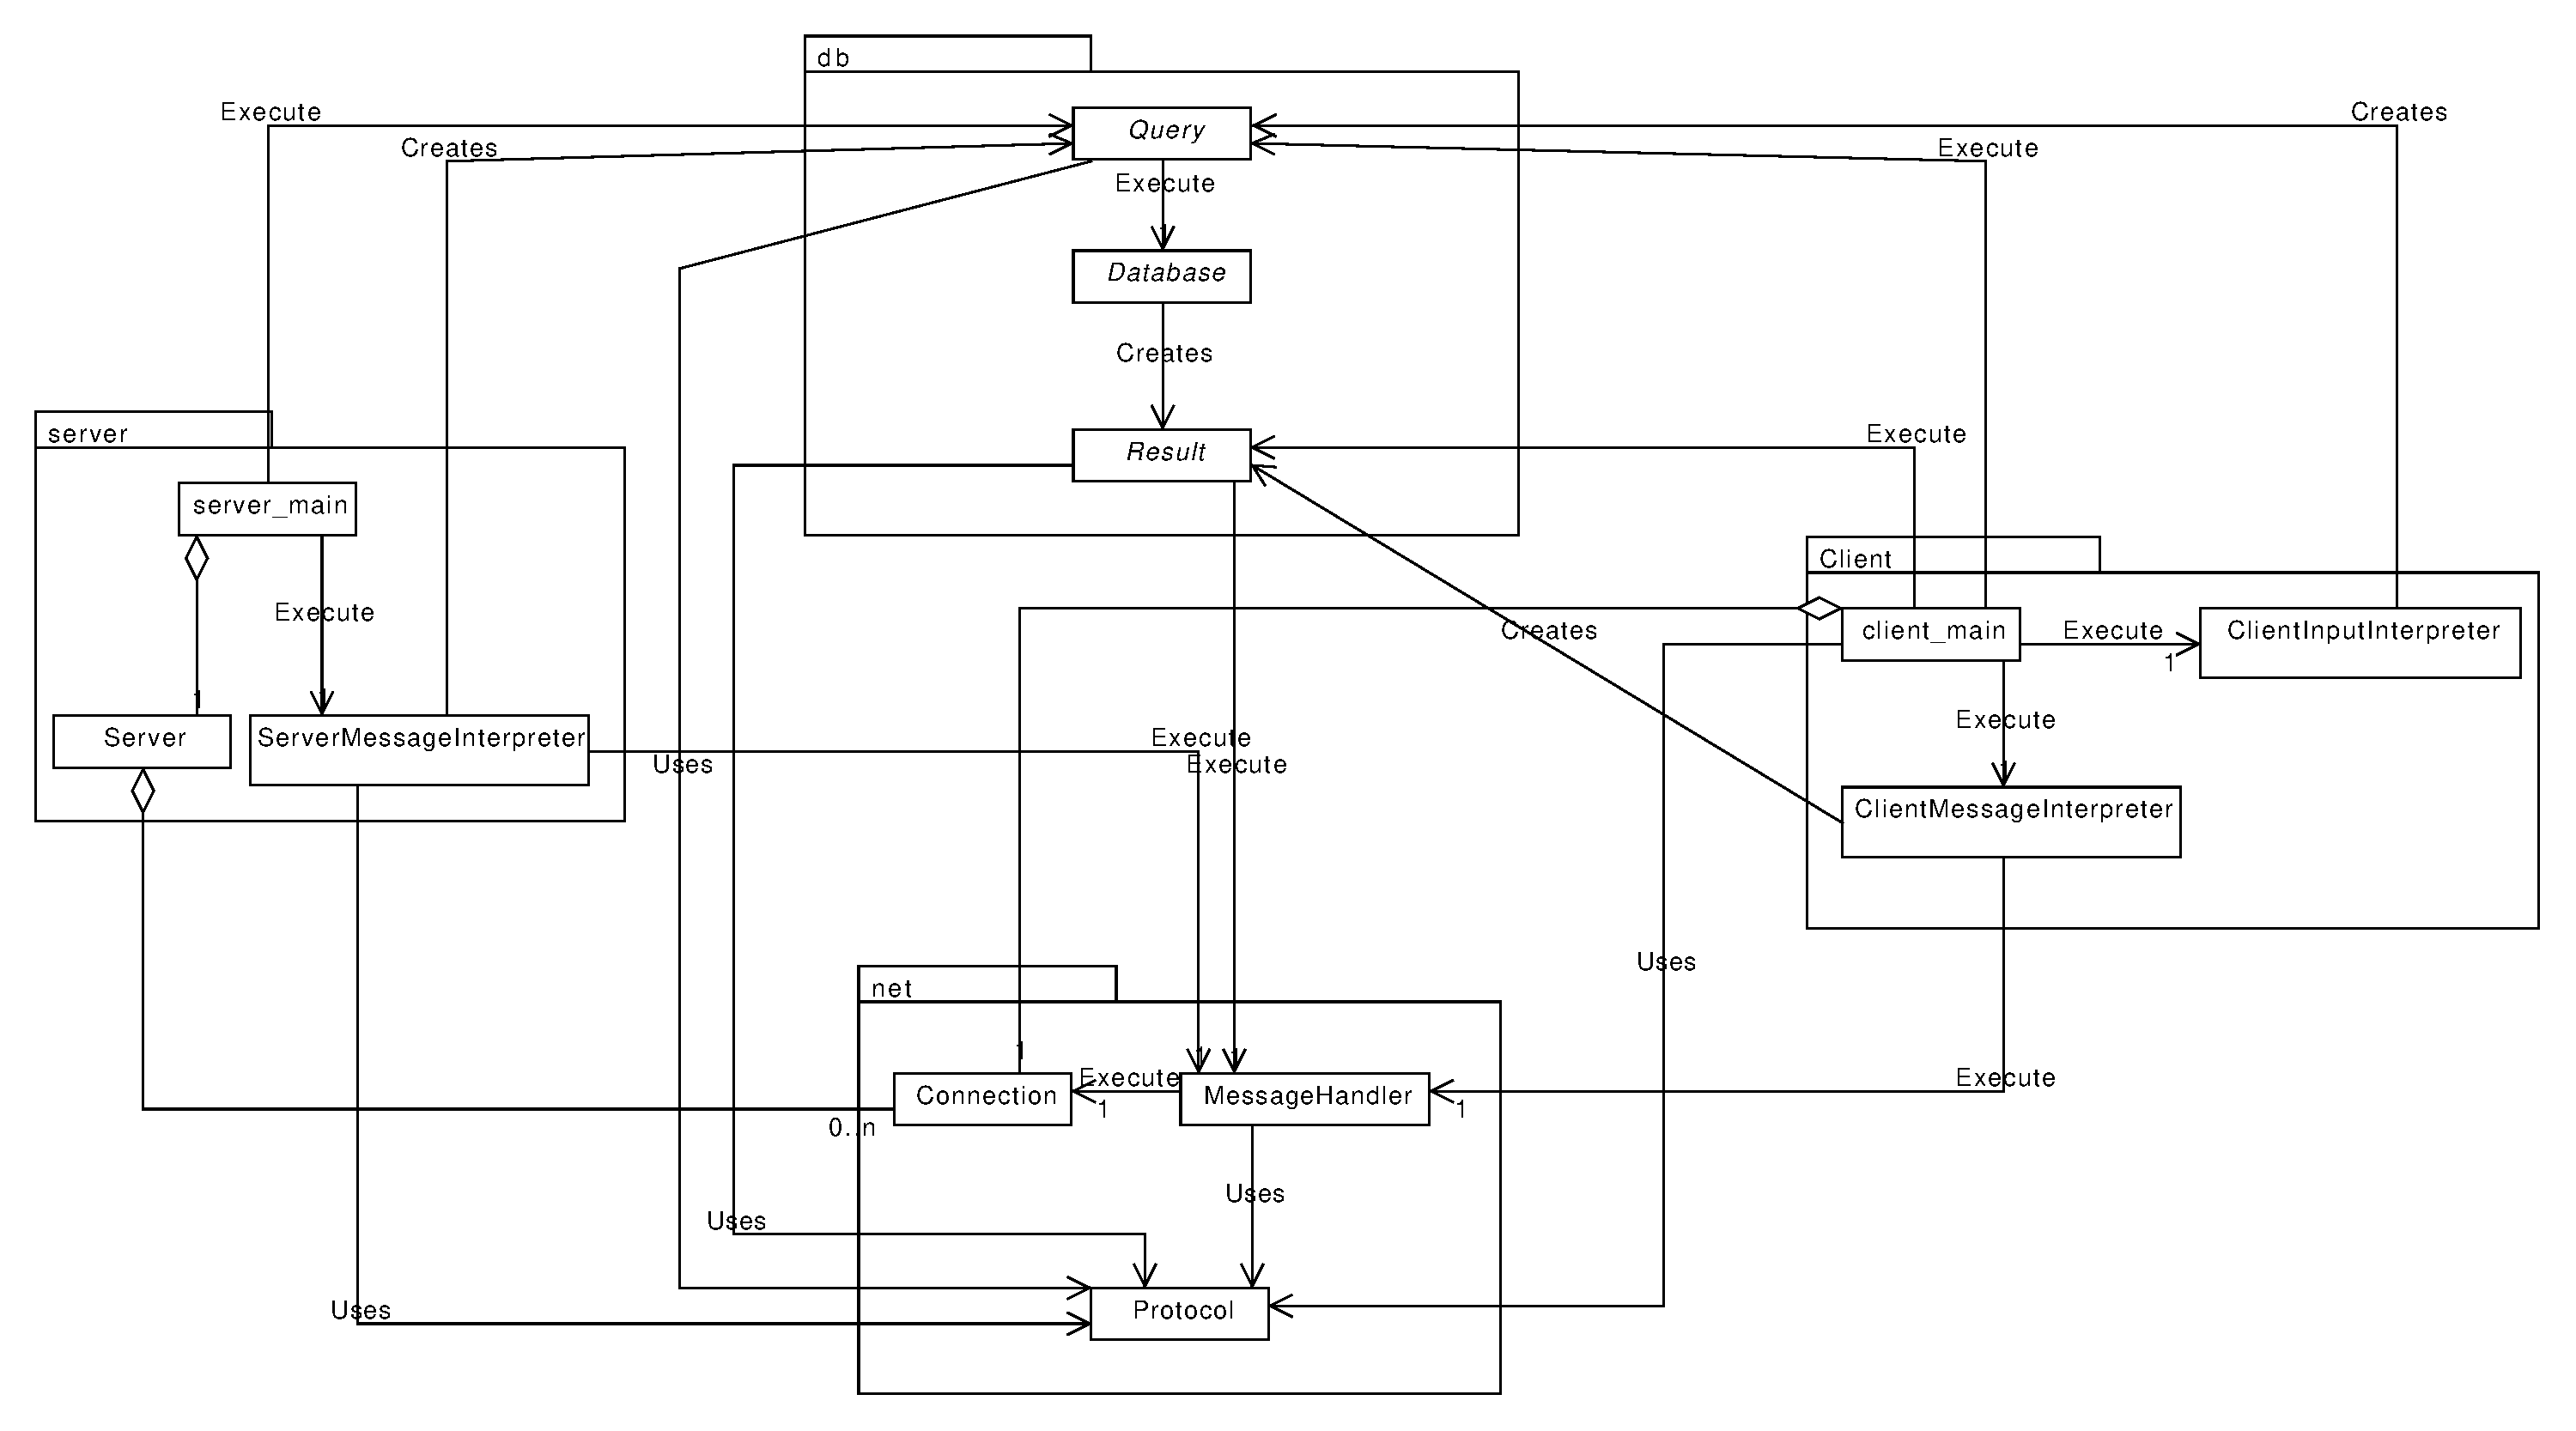
\includegraphics[scale=0.3]{img/uml.pdf}
\end{center}
\label{UML}
\caption{An UML diagram describing the project.}
\end{figure}

\subsection{Net}
Most of the functions needed for using UNIX sockets were given to use from the beginning. We did not need to change them, only put them in this package. The reason for this is probably that the projects goal was to practice C++ and STL, not UNIX programming.

\subsection{DB}
The main purpose of this package is to handle everything involving the database. There are two different types of databases \emph{MemoryDB} and \emph{FileFB}. The memory database stores all the data in memory and destroys it when the server is killed. The file database stores all the data to the file system. The file database must be able to read, create and delete files. For this purpose, the class \emph{db/directory.cc} is used.

The package also contains \emph{Query} and \emph{Result} classes. For every possible query the client sends to the server, there is a corresponding subclass to \emph{Query}. Same thing for the result, for every result the server returns to the client, there is a corresponding subclass to \emph{Result}. The objective of \emph{Query} is to store a query, which can be sent from the client to the server by using \emph{MessageHandler}. The query can be recreated in the server and used to get results from the database. The objective of \emph{Result} is to get data from the database. This result is sent from the server to the client by using \emph{MessageHandler}. The result can then be recreated and made to a string in the client.

\subsection{Client}
The client package contains the client part of the project. The most important class here is \emph{client/client\_main} which starts the client program. First, the program connects itself to a server by using the \emph{Connection} class. It then waits for an input from the user. When it receives a command, the class \emph{ClientInputInterpreter} is involved. This class interprets the command, creates a \emph{Query} object and returns it. The query is then converted to a message and sent to the server by using \emph{MessageHandler} and the \emph{Protocol} class. The result from the server is then received and interpreted by \emph{ClientMessageInterpreter} using \emph{MessageHandler} and returns a \emph{Result} object. The data in this result object is then printed to standard output. This whole process is repeated until the user gives the input \cite{'exit'}.

\subsection{Server}
The server package consists most importantly of the main function found in \emph{server/server\_main}. It first register it self as listener at a port in the operating system. It then wait for events of two types, new connections, disconnections and command requests from existing connections. In the first case the connection is stored, in the second deregistered. In the third case when a request is made the class \emph{ServerMessageInterpreter} is invoked. It knows how to receive queries and used the protocol \emph{net/protocol.h} and the \emph{MessagHandler} to construct a \emph{Query} object. The query is then executed against the database interface which returns a \emph{Result} object. That result knows it data and thus sends it self on the network using a \emph{MessageHandler} for data conversion. We decided to centralize the execution path to the main while loop so we easily could handle exceptions.

\subsection{Communication, flow-chart}
To give an overview of the dynamics of the system we will trace the execution path from when the server receives a command to it sends a reply;

\begin{enumerate}
	\item When a client sends a command to the server it is blocked in \emph{Server::waitForActivity()}, more specifically at the system call \emph{accept()}. In this case it returns with a previously connected client and the function will return a pointer to that connection.
	\item Back at the caller, the while(forever) loop in \emph{server/server\_main.cc}, a \emph{MessageHandler} for this connection in created. The next step is to get an \emph{Query} instance. Thus \emph{MessageInterpreter::receive\_query()} is called with this connection.
	\item It reads the first byte which determines the type of the command. From this a private helper function for that message type is called who will read more bytes from the stream using the \emph{MessageHandler} and interpret them according to the protocol. If this fails an exception will be thrown at caught in the main while loop and the client will be disconnected. Otherwise a derived class of base type \emph{Query} will be instantiated representing the request.
	\item The main while loop will now execute the query with \emph{Query::execute()} of an instance of the database interface. Let this be a \emph{FileDB} since this is the most interesting case.
	\item The query calls the correct function in the database with the parameters for the request stored as members of this object. Let the query be a article listing query since this is a typical usage of the database. In this case \emph{FileDB::list\_art()} is called.
	\item First it must be verified that the news group exists. Therefor a private member function \emph{FileDB::get\_ng()} is called. This function will first need to get a set of news group from the file system so it calls another private member function \emph{FileDB::read\_ngs}. The news groups are stored as directories with their ID as the name. Since each news group must not impose any restrictions on its title that can not be saved as part of the name since a typical file system limits filenames to 255 bytes. The file names are stored in a file \emph{FileDB::DB\_INFO\_NAME} which is scanned for news groups. The result is returned to the \emph{get\_ng} function which will search the result for the requested news group.
	\item Back in the function \emph{list\_ng} we now want to get the articles for the found news group and the function \emph{FileNG::list\_arts()} is called.
	\item The articles are stored with their ID as filename and their title in the first line of the file. First the directory content must be listed which is done by calling \emph{Directory::list\_files()}. That function will call a private function \emph{Directory::list\_type()} with the parameter set to list regular files only.
	\item The file listing is achieved using a pair of \emph{DireIterator}s. In the function \emph{Directory::begin()} a new \emph{DirIterator} is instantiated with the result from the private function \emph{Directory::open\_dir()} which will open the news group directory and return a pointer to a structure representing the opened directory.
	\item The iterator will be incremented causing the next file to be read and dereferenced yielding a pointer to a representation of an entity (file). All file names are collected and returned to \emph{Directory::list\_files} who just passes that up to \emph{FileNG::list\_arts()}. Now a file stream for all files are opened so the IDs can matched with the corresponding article title found in the file. The result is returned to \emph{FileDB::list\_art()}
	\item Now all IDs and  titles can be used to create an \emph{ListArtResult} object.  That is returned to the caller, the query. The query just passes the result up to the main while loop.
	\item Now the result should be sent to the client so the function \emph{Result::printToConnection()} is called with the \emph{MessageHandler}. That function send the result accordingly to the protocol.
	\item The main loop will now restart by waiting for activity on the socket.
	
\end{enumerate}

\subsection{Conclusion}


We also took the chance of trying the front end clang to LLVM after an inspiring guest lecture by Hans Wennborg in the course. We found that it was easier to work with since it produced cleaner and colored output. It also gave useful suggestions to causes and solution to the problems.

\subsubsection{Implemented requirements}

\subsubsection{Problems}
This was our first project developed with C++ and could potentially caused us many problems. However it went surprisingly well and there were relative few problems. We had previous experience from the tools used like GCC, GNU Make, valgrind etc. One obstacle though was to make good Makefile. We wanted all compiled files to be put in a build directory and thus not pollute the source tree. That is fairly simple, just change the path with pattern substitution. But we also wanted to have automatic generation of dependencies so we don't have to update the Makefile each time we include something new. Thus we want a Makefile for each .cc-file. Examples on how to do that have been used in the course and take from the GNU Make manual section 4.4 \cite{makeman}. Also we wanted the structure on disk to reflect the programs logical division in namespaces.

However the combination separate output directory, automatic prerequisites generation and structural directories proved to be a daunting task. After days of hacking, manual consultation and testing it was found that the automatic compilation targets for .cc-files to .o-files that the solution from the manpages was never invoked when the target destination is not the same as the prerequisite. This had to be solved with some really ugly hacks but we got it working. At least we are now eager to start using tools from the GNU build system or CMake to escape the task of writing Makefiles.


\subsubsection{Missing features}
We believe that we have implemented all features outlined in the specification.

\subsubsection{Suggestions}




\emph{\cite{dummy+ref}} 
\newpage
\bibliographystyle{plain}
\bibliography{references}
\end{document}

%\begin{figure}[hbt]
%\begin{center}
%\includegraphics[scale=0.4]{img/pic1.png}
%\end{center}
%\label{LABEL}
%\caption{DESCRIPTION text.}
%\end{figure}
%\clearpage

%\VerbatimInput{src/prog1.c}
